\documentclass[../../main.tex]{subfiles}

    \lstset{basicstyle=\small,
      showstringspaces=false,
      commentstyle=\color{black},
      keywordstyle=\color{blue}
    }

    \graphicspath{{images/Konzepte/}{../../images/Konzepte/}}


    \begin{document}
    \subsection{Software TinyK22} \label{et_software_tiny}
    Dieses Kapitel beschreibt die Software, welche auf dem Mikrocontroller TinyK22 implementiert ist. Diese Software kommuniziert mit mit dem Pi und steuert die nötigen Sensoren und aktoren an. Die Schnittstelle zum Pi ist in Kapitel \ref{interface_pi_tiny} beschrieben. Weiteres Angaben zu den Sensoren und Aktoren und deren elektrische Verbindungen sind in Kapitel \ref{et_verbindungen} und \ref{et_Komponenten}.\\
    Die Software auf dem Mikrocontroller wird gemäss \ref{tab:et_mc_softwarekonzept} in verschiedene Module unterteilt.\\

    \begin{table}[H]
        \centering
        \begin{tabular}{|l|p{12cm}|}
        \hline
        \textbf{Modulname} & \textbf{Beschreibung}    \\ \hline
        com   & Kommunikation mit dem pi                                                                                 \\ \hline
        cube  & Würfelerkennung mit Ansteuerung des TOF Sensors über I2C                                                 \\ \hline
        drive & Ansteuerung des Antriebmotors mit Regelung der Geschwindigkeit mittels dem Feedback vom Quadraturencoder \\ \hline
        crane & Ansteuerung des Motors für den Schwenker mit Positionsregelung mittels dem Feedback vom Quadraturencoder \\ \hline
        \end{tabular}
        \caption{Module Software TinyK22}
        \label{tab:et_mc_softwarekonzept}
        \end{table}


    In Abbildung \ref{fig:et_mc_softwarekonzept} ist die Aufteilung veranschaulicht. Mit grün sind jeweisl die einzelnen Module gekennzeichnet. Die Module benutzen jeweils ihre Komponenten abwärts bis zum Zugriff auf die Hardware. In Abbildung \ref{fig:et_mc_softwarekonzept} gelb gekennzeichnet repräsentiert die Komponenten, welche auf die Hardware des Mikrocontrollers zugreifen. Orange kennzeichnet die Komponenten, welche als Schnittstellen zwischen dem Hardwarezugriff und der Logik dienen. Diese Bereiten Informationen der Hardware auf in ein Format, dass die Logik gut verarbeiten kann. Die Logik ist in den rot gekennzeichneten Komponenten implementiert. Diese verarbeitet die Daten und trifft Entscheidungen.
    In Abbildung \ref{fig:et_mc_softwarekonzept} aus Übersichtsgründen nicht ersichtlich ist, dass alle module auf das com modul zugreifen können um mit dem Pi zu kommunizieren. Dabei benützen die Module die Komponenten comPi, comAck und comLog.\\

    \begin{figure}[H]
        \centering
        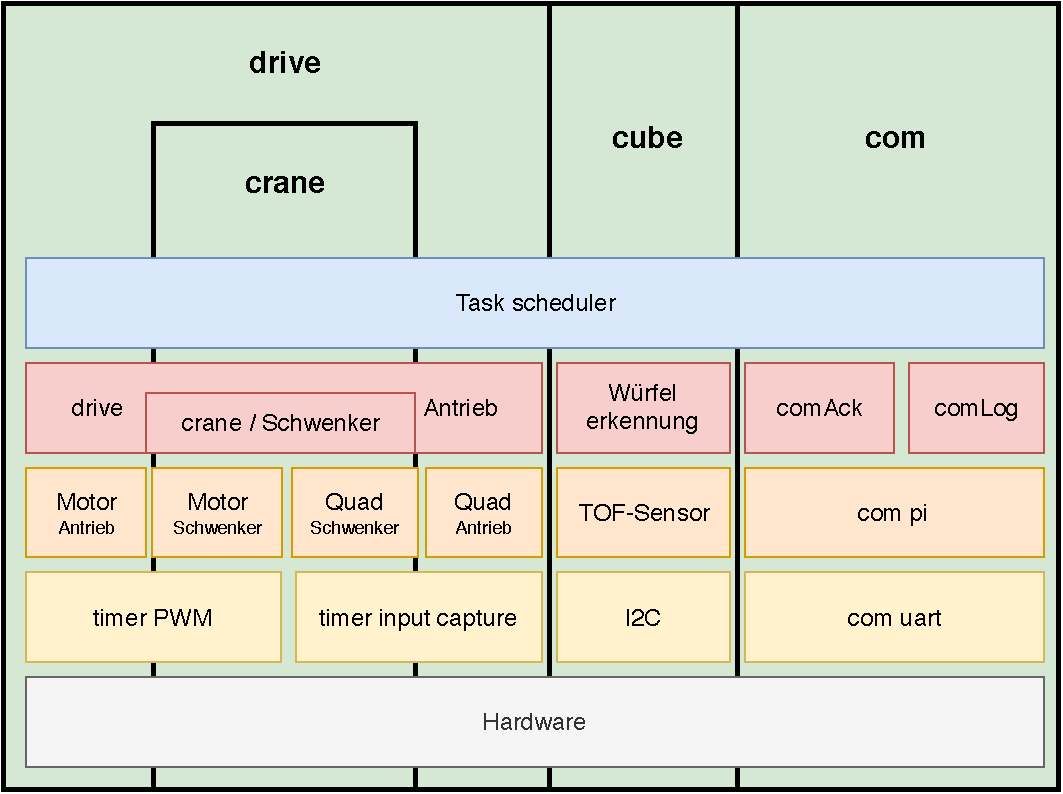
\includegraphics[width=1.0\textwidth]{../../images/et/et_mc_softwarekonzept.pdf}
        \caption {Modulaufteilung TinyK22}
        \label{fig:et_mc_softwarekonzept}
    \end{figure}

    \begin{wrapfigure}{r}{0.3\textwidth}
        \centering
        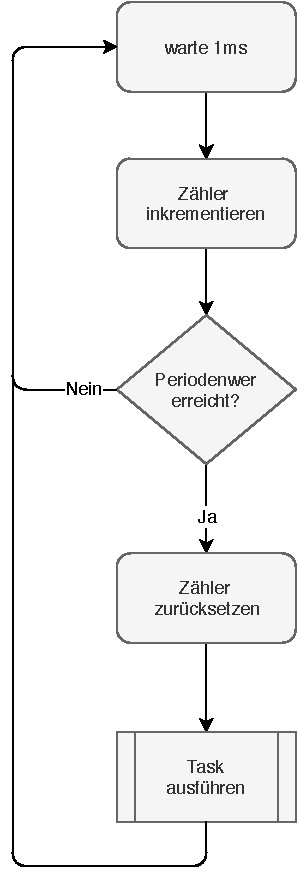
\includegraphics[width=0.3\textwidth]{../../images/et/et_task_scheudler.pdf}
        \caption {Flussdiagramm Task Scheudler}
        \label{fig:et_task_scheudler}
    \end{wrapfigure}

    Für jedes Modul gibt es eine Taskfunktion, die während des Betriebs in einem Task Scheduler Loop periodisch aufgerufen wird. Auf die Benutzung eines Betriebssysteme wurde in diesem Projekt verzichtet. Der es gibt also keine Prioritäten oder Time-Slicing für die Tasks. Abbildung \ref{fig:et_task_scheudler} veranschaulicht das Prinzip der Implementation für einen Task. Wichtig dabei zu beachten ist, dass mit dieser Variante die vorgegebenen Zeitintervalle nicht exakt und je nach Auslastung variieren. Da die Tasks aber ohnehin nicht stark zeitkritisch sind funktioniert dies trotzdem. Alle Zeitkritischen Aufgaben werden über Interrupts behandelt.

    \subsubsection{Modul com}

    \subsubsection{Modul cube}
    
    \subsubsection{Modul drive}

    \subsubsection{Modul crane}

    \end{document}